% SECTION: Gaussian Mixture Models (GMMs)
\section{Gaussian Mixture Models (GMMs)}

\divider

% SUBSECTION: Problemstellung
\subsection{Problemstellung}

% Problemstellung
\begin{frame}{Problemstellung}{}
	\begin{itemize}
		\item Wir wissen bereits, wie wir die Parameter $\bmu$ und $\bSigma$ einer Normalverteilung aus Daten schätzen.
		\item Wiederholung: \textbf{Maximum-Likelihood Lösung}
		\begin{itemize}
			\item Gegeben sei ein Datensatz $\bX$ bestehend aus $N$ unabhängig und identisch normalverteilten Punkten
				$\bx_1, \bx_2, \ldots, \bx_N$.
			\item Schätze den Mittelwert $\bmu$ gemäß
			\begin{equation}
				\bmuML \coloneqq \frac{1}{N} \sum_{n=1}^N \bx_n.
			\end{equation}
			\item Schätze die Kovarianzmatrix $\bSigma$ mittels
			\begin{equation}
				\bSigmaML \coloneqq \frac{1}{N} \sum_{n=1}^N \bigl( \bx_n - \bmuML \bigr) \bigl( \bx_n - \bmuML \bigr)^\top.
			\end{equation}
		\end{itemize}
		\item \textbf{Frage:} Wie gehen wir mit multimodalen Daten um?
	\end{itemize}
\end{frame}


% Visualisierung: Problemstellung
\begin{frame}{Visualisierung: Problemstellung}{}
	\begin{figure}
		\centering
		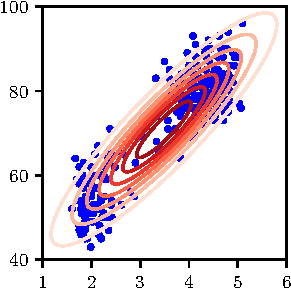
\includegraphics[scale=1.00]{./img/gmm/one_gaussian}
		\caption{Modell bestehend aus einer Normalverteilung. Siehe \cite{Bishop2024}, Seite 86.}
	\end{figure}
\end{frame}


% Visualisierung: Problemstellung (Forts.)
\begin{frame}{Visualisierung: Problemstellung (Forts.)}{}
	\begin{figure}
		\centering
		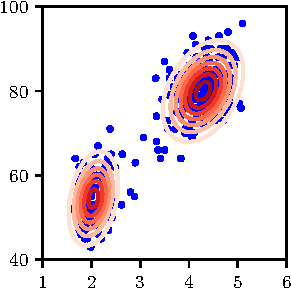
\includegraphics[scale=1.00]{./img/gmm/gaussian_mixture}
		\caption{Mixture Modell bestehend aus zwei Normalverteilungen. Siehe \cite{Bishop2024}, Seite 86.}
	\end{figure}
\end{frame}


% Gaussian Mixture Models
\begin{frame}{Gaussian Mixture Models}{}
	\begin{itemize}
		\item Wir können ein \keyword{Gaussian Mixture Model} als eine \textit{Überlagerung mehrerer Normalverteilungen} ansehen.
		\item Die Dichte bei $K$ Komponenten ist gegeben durch
		\begin{equation}
		\label{eq:gmm-density}
			p(\bx) \coloneqq \sum_{k=1}^K \pi_k \cdot \norm(\bx; \bmu_k, \bSigma_k).
		\end{equation}
		\item Die \keyword{Mischkoeffizienten} $\pi_k$ stellen sicher, dass die Mixture-Dichte normiert ist,
			sodass also $\int_{-\infty}^{+\infty} p(\bx) = 1$ gilt.
		\item Die $\pi_k$ erfüllen zudem
		\begin{equation*}
			0 \le \pi_k \le 1
		\qquad\text{und}\qquad
			\sum_{k=1}^K \pi_k = 1.
		\end{equation*}
	\end{itemize}
\end{frame}


% Gaussian Mixture Models als Latent Variable Models
\begin{frame}{Gaussian Mixture Models als Latent Variable Models}{}
	\begin{itemize}
		\item Sei im Folgenden $\bz \in \R^K$ ein $K$-dimensionaler \keyword{One-Hot Vektor}.
		\item Die Komponenten $z_k$ erfüllen also $z_k \in \{ 0, 1 \}$ und $\sum_{k=1}^K z_k = 1$,
			wobei \textit{genau eine Komponente} den Wert 1 annimmt.
		\item Wir definieren nun die gemeinsame Verteilung von $\bx$ und $\bz$ über die Kettenregel
		\begin{equation*}
			p(\bx, \bz) = p(\bx \mid \bz) \cdot p(\bz).
		\end{equation*}
		\item Für die Definition der Randverteilung $p(\bz)$ benutzen wir die Mischkoeffizienten: $p(z_k = 1) \coloneqq \pi_k$.
		\item Da $\bz$ ein One-Hot Vektor ist, können wir schreiben
		\begin{equation}
		\label{eq:gmm-marginal-z}
			p(\bz) = \prod_{k=1}^K \pi_k^{z_k}.
		\end{equation}
	\end{itemize}
\end{frame}


% Gaussian Mixture Models als Latent Variable Models (Forts.)
\begin{frame}{Gaussian Mixture Models als Latent Variable Models (Forts.)}{}
	\begin{itemize}
		\item Analog definieren wir
		\begin{equation*}
			p(\bx \mid z_k = 1) \coloneqq \norm(\bx; \bmu_k, \bSigma_k).
		\end{equation*}
		\item Dies können wir ebenfalls vektorisiert ausdrücken als
		\begin{equation}
		\label{eq:gmm-x-given-z}
			p(\bx \mid \bz) \coloneqq \prod_{k=1}^K \norm(\bx; \bmu_k, \bSigma_k)^{z_k}.
		\end{equation}
		\item Die Randverteilung $p(\bx)$ erhalten wir schließlich, indem wir über alle möglichen Werte $\bz$ summieren
		\begin{equation}
			p(\bx) = \sum_{\bz} p(\bz) \cdot p(\bx \mid \bz) = \sum_{k=1}^K \pi_k \cdot \norm(\bx; \bmu_k, \bSigma_k).
		\end{equation}
		\item Im letzten Gleichheitszeichen haben wir \eqref{eq:gmm-marginal-z} und \eqref{eq:gmm-x-given-z}
			zusammen mit der One-Hot Eigenschaft von $\bz$ benutzt.
	\end{itemize}
\end{frame}


% Latente Variablen
\begin{frame}{Latente Variablen}{}
	\begin{itemize}
		\item Falls ein Datensatz $\bX$ bestehend aus $N$ Punkten $\bx_1, \bx_2, \ldots, \bx_N$ vorliegt, so führen wir
			für jedes $\bx_n$ ein entsprechendes $\bz_n$ ein.
		\item Die Variablen $\bz_n$ nennt man \keyword{latent}, da man sie nicht beobachtet.
		\item Sei $\bz_n$ die latente Variable für Punkt $\bx_n$.
		\item Die Aussage $z_{nk} = 1$ bedeutet dann, dass $\bx_n$ von Komponente $k$ generiert wurde.
		\item Auf den ersten Blick wirkt die Einführung zusätzlicher Variablen nicht zielführend.
		\item Allerdings können wir nun mit der Verteilung $p(\bx, \bz)$ anstelle von $p(\bx)$ arbeiten,
			was zu wesentlichen Vereinfachungen führen wird.
		\item Insbesondere kann der \keyword{Expectation-Maximization (EM) Algorithmus} verwendet werden \\
			(siehe nächstes Kapitel).
	\end{itemize}
\end{frame}


% Responsibilities
\begin{frame}{Responsibilities}{}
	\begin{itemize}
		\item Im weiteren Verlauf interessieren wir uns besonders für die Aposteriori-Wahrscheinlichkeit $p(\bz \mid \bx)$.
		\item Mit $\gamma(z_k)$ bezeichnen wir die Wahrscheinlichkeit $p(z_k = 1 \mid \bx)$.
		\item Mit dem \textit{Satz von Bayes} gilt
		\begin{align*}
			\gamma(z_k) \coloneqq p(z_k = 1 \mid \bx)
				&= \frac{p(z_k = 1) \cdot p(\bx \mid z_k = 1)}{\sum_{j=1}^K p(z_j = 1) \cdot p(\bx \mid z_j = 1)}
		\\[2mm]
				&= \frac{\pi_k \cdot \norm(\bx; \bmu_k, \bSigma_k)}{\sum_{j=1}^K \pi_j \cdot \norm(\bx; \bmu_j, \bSigma_j)}.
		\end{align*}
		\item In diesem Zusammenhang ist $\pi_k$ die Apriori-Wahrscheinlichkeit für $z_k = 1$ und
			$\gamma(z_k)$ die Aposteriori-Wahrscheinlichkeit für $z_k = 1$, nachdem $\bx$ beobachtet wurde.
		\item Man nennt $\gamma(z_k)$ auch die \keyword{Responsibility} der $k$-ten Komponente für Punkt $\bx$. 
	\end{itemize}
\end{frame}


% Visualisierung: Responsibilities
\begin{frame}{Visualisierung: Responsibilities}{}
	\begin{figure}[H]
		\begin{minipage}[t]{0.3\textwidth}
			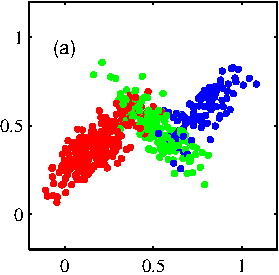
\includegraphics[scale=0.85]{./img/gmm/gmm_data_generation}
		\end{minipage}
		\hfill
		\begin{minipage}[t]{0.3\textwidth}
			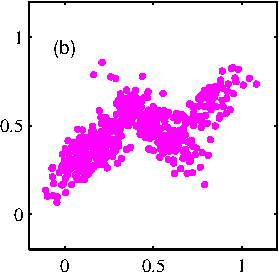
\includegraphics[scale=0.85]{./img/gmm/gmm_data_generation_wo_labels}
		\end{minipage}
		\hfill
		\begin{minipage}[t]{0.3\textwidth}
			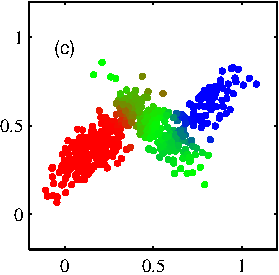
\includegraphics[scale=0.85]{./img/gmm/gmm_responsibilities}
		\end{minipage}
		\caption{(a) Beispiel von 500 Punkten, die von drei verschiedenen Normalverteilungen stammen.
		(b) Datensatz ohne die Information, von welcher Verteilung die Daten stammen.
		(c) Plot der Responsibilities. Dabei wurden die Farben im Verhältnis der Wahrscheinlichkeiten
		$\gamma(z_nk)$ gewählt. Siehe \cite{Bishop2024}, Seite 469.}
	\end{figure}
\end{frame}


% Likelihood Funktion
\begin{frame}{Likelihood Funktion}{}
	\begin{itemize}
		\item Im Folgenden sei ein Datensatz bestehend aus $N$ unabhängigen und identisch verteilten Punkten $\bx_1, \bx_2, \ldots, \bx_N$ gegeben.
		\item Wir fassen die Punkte $\bx_n$, $n = 1, 2, \ldots$ in der Matrix $\bX \in \R^{N \times M}$ zusammen,
			wobei die $n$-te Zeile durch $\bx_n^\top$ gegeben ist.
		\item Mit \eqref{eq:gmm-density} ergibt sich die Log-Likelihood Funktion des Mixture Models zu
		\begin{align*}
			\ln p(\bX; \bpi, \bmu, \bSigma)
				&= \ln\left( \prod_{n=1}^N \left( \sum_{k=1}^K \pi_k \cdot \norm(\bx_n \mid \bmu_k, \bSigma_k) \right) \right)
		\\[2mm]
				&= \sum_{n=1}^N \ln\left( \sum_{k=1}^K \pi_k \cdot \norm(\bx_n \mid \bmu_k, \bSigma_k) \right).
		\end{align*}
		\item Aufgrund der Summe im Argument des Logarithmus ist dieser Ausdruck schwer zu optimieren.
	\end{itemize}
\end{frame}


% Gradient der Log-Likelihood für die Mittelwerte
\begin{frame}{Gradient der Log-Likelihood für die Mittelwerte}{}
	\vspace*{-10mm}
	\begin{align*}
		\frac{\partial}{\partial \bmu_k} \ln p(\bX; \bpi, \bmu, \bSigma)
			&= \sum_{n=1}^N \frac{1}{p(\bx_n; \bpi, \bmu, \bSigma)} \cdot \frac{\partial}{\partial \bmu_k} p(\bx_n; \bpi, \bmu, \bSigma)
	\\[2mm]
			&= \sum_{n=1}^N \left( \frac{1}{p(\bx_n; \bpi, \bmu, \bSigma)} \cdot
				\sum_{j=1}^K \pi_j \frac{\partial}{\partial \bmu_k} \norm(\bx_n; \bmu_j, \bSigma_j) \right)
	\\[2mm]
			&= \sum_{n=1}^N \frac{\pi_k}{p(\bx_n; \bpi, \bmu, \bSigma)} \cdot
				\frac{\partial}{\partial \bmu_k} \norm(\bx_n; \bmu_k, \bSigma_k)
	\\[2mm]
			&= \sum_{n=1}^N \frac{\pi_k \cdot \norm(\bx_n; \bmu_k, \bSigma_k)}{\sum_{j=1}^K \pi_j \cdot \norm(\bx_n; \bmu_j, \bSigma_j)} \cdot
				\bSigma_k^{-1} (\bx_n - \bmu_k)
	\\[2mm]
			&= \sum_{n=1}^N \gamma(z_{nk}) \cdot \bSigma_k^{-1} (\bx_n - \bmu_k)
	\end{align*}
\end{frame}


% Lösung für die Mittelwerte
\begin{frame}{Lösung für die Mittelwerte}{}
	\begin{itemize}
		\item Wir setzen diesen Ausdruck Null und lösen nach $\bmu_k$ auf
		\begin{equation*}
			\sum_{n=1}^N \gamma(z_{nk}) \cdot \bSigma_k^{-1} (\bx_n - \bmu_k) \overset{!}{=} 0
		\quad\Longleftrightarrow\quad
			\bmu_k = \frac{1}{N_k} \sum_{n=1}^N \gamma(z_{nk}) \cdot \bx_n.
		\end{equation*}
		\item Hierbei ist $$N_k \coloneqq \sum_{n=1}^N \gamma(z_{nk})$$ die Summe der Responsibilities der $k$-ten Komponente.
		\item Der Mittelwert $\mu_k$ der $k$-ten Komponente ergibt sich also durch ein \textit{gewichtetes arithmetisches Mittel},
			wobei die Gewichtungsfaktoren gerade die Aposteriori-Wahrscheinlichkeiten dafür sind,
			dass $\bx_n$ durch die $k$-te Komponente generiert wurde.
	\end{itemize}
\end{frame}


% Lösung für die Kovarianzmatrizen
\begin{frame}{Lösung für die Kovarianzmatrizen}{}
	\begin{itemize}
		\item Ein ähnliches Ergebnis erhalten wir für die Kovarianzmatrizen $\bSigma_k$.
		\item Es ist
		\begin{equation}
			\bSigma_k = \frac{1}{N_k} \sum_{n=1}^N \gamma(z_{nk}) \cdot (\bx_n - \bmu_k) (\bx_n - \bmu_k)^\top.
		\end{equation}
		\item Auch hier ergeben sich die Parameter als gewichtetes arithmetisches Mittel.
	\end{itemize}
	
	\begin{mytask}
		Beweisen Sie diese Aussasge!
	\end{mytask}
\end{frame}


% Optimierung bezüglich der Mischkoeffizienten
\begin{frame}{Optimierung bezüglich der Mischkoeffizienten}{}
	\begin{itemize}
		\item Hier müssen wir bei der Optimierung zusätzlich beachten, dass $\sum_{k=1}^K \pi_k = 1$ erfüllt sein muss.
		\item Es handelt sich also um ein \textit{restringiertes Optimierungsproblem}.
		\item Die Lagrange-Funktion ist
		\begin{align*}
			\lagrange
				&= \ln p(\bX; \bpi, \bmu, \bSigma) + \lambda\left( \sum_{k=1}^K \pi_k - 1 \right)
		\\[2mm]
				&= \sum_{n=1}^N \ln\left( \sum_{k=1}^K \pi_k \cdot \norm(\bx_n \mid \bmu_k, \bSigma_k) \right)
					+ \lambda\left( \sum_{k=1}^K \pi_k - 1 \right)
		\end{align*}
	\end{itemize}
\end{frame}


% Gradient der Log-Likelihood für die Mischkoeffizienten
\begin{frame}{Gradient der Log-Likelihood für die Mischkoeffizienten}{}
	\vspace*{-8mm}
	\begin{align*}
		\frac{\partial\lagrange}{\partial \pi_k}
			&= \frac{\partial}{\partial \pi_k} \ln p(\bX; \bpi, \bmu, \bSigma)
				+ \lambda \cdot \frac{\partial}{\partial \pi_k} \left( \sum_{k=1}^K \pi_k - 1 \right)
	\\[2mm]
			&= \sum_{n=1}^N \frac{1}{p(\bx_n; \bpi, \bmu, \bSigma)} \cdot \frac{\partial}{\partial \pi_k} p(\bx_n; \bpi, \bmu, \bSigma) + \lambda
	\\[2mm]
			&= \frac{1}{\pi_k} \sum_{n=1}^N \frac{\pi_k \cdot \norm(\bx_n; \bmu_k, \bSigma_k)}{
				\sum_{j=1}^K \pi_j \cdot \norm(\bx_n; \bmu_j, \bSigma_j)
			} + \lambda
	\\[2mm]
			&= \frac{1}{\pi_k} \sum_{n=1}^N \gamma(z_{nk}) + \lambda
	\\[2mm]
			&= \frac{N_k}{\pi_k} + \lambda
	\end{align*}
\end{frame}


% Lösung für die Mischkoeffizienten
\begin{frame}{Lösung für die Mischkoeffizienten}{}
	\begin{itemize}
		\item Zusätzlich benötigen wir noch die Ableitung nach $\lambda$
		\begin{equation*}
			\frac{\partial\lagrange}{\partial\lambda} = \sum_{k=1}^K \pi_k - 1.
		\end{equation*}
		\item Setzen wir beide Gleichungen Null, so erhalten wir
		\begin{equation*}
			\pi_k = -\frac{N_k}{\lambda}
		\quad\text{und}\quad
			1 = \sum_{k=1}^K \pi_k.
		\end{equation*}
		\item Setzen wir die erste Bedingung in die zweite ein, so erhalten wir $\lambda = -N$ und damit schließlich
		\begin{equation}
			\pi_k = \frac{N_k}{N}.
		\end{equation}
	\end{itemize}
\end{frame}


% Expectation-Maximization (EM) Algorithmus für GMMs
\begin{frame}{Expectation-Maximization (EM) Algorithmus für GMMs}{}
	\begin{itemize}
		\item Bei den Lösungsformeln handelt es sich \textit{nicht um geschlossene Lösungsformeln}, da die Gewichte $\gamma(z_{nk})$ von den anderen
			Parametern abhängen.
		\item Allerdings legen die Ergebnisse ein einfaches iteratives Verfahren nahe, den \keyword{Expectation-Maximization (EM) Algorithmus}.
		\item Dieser besteht aus zwei Phasen, die \keyword{Expectation-Phase (E-Schritt)} und die \keyword{Maximization-Phase (M-Schritt)}.
		\item Im E-Schritt werden die Werte $\gamma(z_{nk})$ bei gegebenen Parametern $\bpi_k, \bmu_k, \bSigma_k$ bestimmt.
		\item Im darauffolgenden M-Schritt werden die Parameter mit den neuen Werten $\gamma(z_{nk})$ aufdatiert.
		\item Dies führt man solange fort, bis Konvergenz eintritt.
	\end{itemize}
\end{frame}


% Visualisierung: EM für GMMs
\begin{frame}{Visualisierung: EM für GMMs}{}
	\begin{figure}[H]
		\begin{minipage}[t]{0.3\textwidth}
			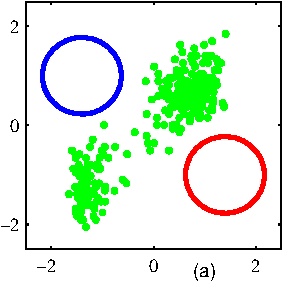
\includegraphics[scale=0.85]{./img/gmm/gmm_em_alg_a}
		\end{minipage}
		\hfill
		\begin{minipage}[t]{0.3\textwidth}
			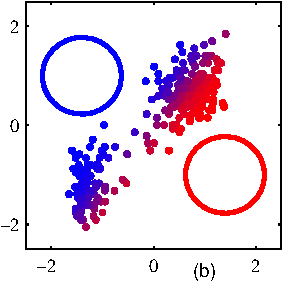
\includegraphics[scale=0.85]{./img/gmm/gmm_em_alg_b}
		\end{minipage}
		\hfill
		\begin{minipage}[t]{0.3\textwidth}
			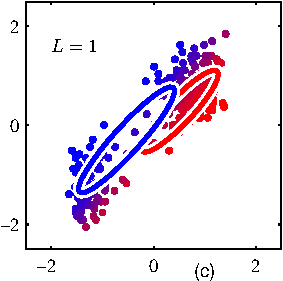
\includegraphics[scale=0.85]{./img/gmm/gmm_em_alg_c}
		\end{minipage}
		\caption{Visualisierung EM für GMMs. Siehe \cite{Bishop2024}, Seite 473.}
	\end{figure}
\end{frame}


% Visualisierung: EM für GMMs (Forts.)
\begin{frame}{Visualisierung: EM für GMMs (Forts.)}{}
	\begin{figure}[H]
		\begin{minipage}[t]{0.3\textwidth}
			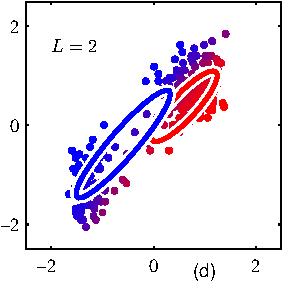
\includegraphics[scale=0.85]{./img/gmm/gmm_em_alg_d}
		\end{minipage}
		\hfill
		\begin{minipage}[t]{0.3\textwidth}
			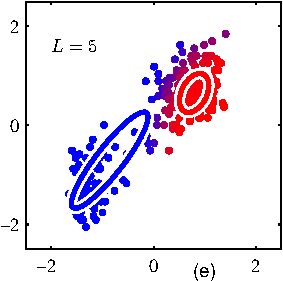
\includegraphics[scale=0.85]{./img/gmm/gmm_em_alg_e}
		\end{minipage}
		\hfill
		\begin{minipage}[t]{0.3\textwidth}
			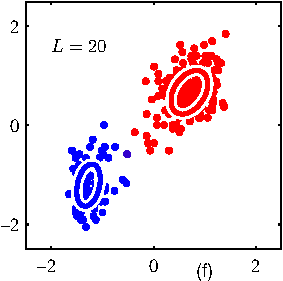
\includegraphics[scale=0.85]{./img/gmm/gmm_em_alg_f}
		\end{minipage}
		\caption{Visualisierung EM für GMMs. Siehe \cite{Bishop2024}, Seite 473.}
	\end{figure}
\end{frame}










































